\documentclass[sigplan,screen,nonacm]{acmart}
\usepackage{rotating}
\usepackage{tabularray}
\usepackage{color}
\setlength {\marginparwidth }{2cm}
\usepackage[colorinlistoftodos]{todonotes}
\usepackage[
    type={CC},
    modifier={by-nc-sa},
    version={4.0},
]{doclicense}

%% \BibTeX command to typeset BibTeX logo in the docs
\AtBeginDocument{%
  \providecommand\BibTeX{{%
    \normalfont B\kern-0.5em{\scshape i\kern-0.25em b}\kern-0.8em\TeX}}}

%% end of the preamble, start of the body of the document source.

\begin{document}

%%
%% The "title" command has an optional parameter,
%% allowing the author to define a "short title" to be used in page headers.
\title[IoT for Wildlife Tracking]{Using Internet of Things for Wildlife Tracking}

%% "authornote" and "authornotemark" commands
%% used to denote shared contribution to the research.
\author{Collin R. Beane}
\email{beane039@morris.umn.edu}
\affiliation{%
  \institution{Division of Science and Mathematics
    \\
    University of Minnesota, Morris
  }
  \city{Morris}
  \state{Minnesota}
  \country{USA}
  \postcode{56267}
}

\begin{abstract}
  The intersection of biologging and Internet of Things (IoT) technologies has revolutionized wildlife tracking, 
  offering unprecedented insights into animal behavior and ecology. This paper provides a comprehensive overview 
  of biologging and IoT concepts, exploring their integration in wildlife tracking applications. We delve into 
  traditional wildlife tracking methods and emerging IoT solutions, analyzing the operational mechanisms, comparative 
  advantages, and limitations of each. Specifically, we examine the use of Low Power Wide Area Networks (LPWAN) such 
  as SigFox and LoRa, alongside traditional WiFi networks, highlighting their respective benefits and considerations 
  in biologging systems. Furthermore, we discuss the critical role of security measures in safeguarding sensitive data 
  transmitted by biologging devices. By elucidating these technologies' capabilities and challenges, this paper aims 
  to provide researchers and conservationists with a framework for evaluating and implementing IoT-enabled biologging 
  systems in ecological research and conservation efforts.
\end{abstract}

\doclicenseThis

\keywords{IoT, networking, data transmission, animal trackers, Sigfox, LoRa, WildFi, Biologging, ecology}


%%
%% This command processes the author and affiliation and title
%% information and builds the first part of the formatted document.
\maketitle

\section{Introduction}
\label{sec:introduction}

The proliferation of the Internet of Things has sparked innovation across various domains, including 
wildlife tracking. Understanding the convergence of biologging and IoT technologies is pivotal in comprehending 
their applications in monitoring animal behavior and ecology. This paper provides a comprehensive overview of 
the foundational concepts behind biologging and IoT, delving into their intersection and exploring the myriad 
technologies employed in wildlife tracking. By examining traditional methods alongside emerging IoT solutions, 
I aim to establish a framework for evaluating the efficacy of IoT-enabled biologging systems in ecological 
research and conservation efforts.

\section{Background}
\label{sec:Background}

Comprehending the foundational technology behind the IoT
is paramount in grasping its applications in wildlife tracking. This section
aims to furnish a concise overview of biologging, IoT, and how data is transmitted 
over wireless networks. Additionally, it will explore current and past
technologies employed in biologging, shedding light on their operational
mechanisms and differences in order to compare them to a modern IoT based biologging 
system.

\subsection{What is Biologging?}
\label{subsec:What is Biologging}

Biologging is a concept that gained popularity in the early 2000's and has continued
to play a pivotal role in understanding animal behavior and ecology. Biologging can be
defined as "The investigation of phenomena in or around free-ranging organisms that are beyond
the boundary of our visibility or experience. \cite{boyd2004bio}" Biologging provides
insights into the behavior and functions of various organisms in environments that
can be hostile or difficult to reach for the observer \cite{boyd2004bio}.
It is a method of tracking animals in the wild using electronic devices that are
attached to the animal. These devices can be used to track the animal's
movements, monitor its behavior, and collect data on its environment. This data
has been used to study animal behavior, migration patterns, and the effects of climate change
on various species \cite{10.3389/fevo.2018.00092}. The data collected from biologging
devices is also useful for informing conservation efforts and helping protect endangered
species \cite{cooke2008biotelemetry}. Importantly, biologging is merely the collection of data, 
and the interpretation of the data is up to the ecologists and conservationists.

\subsection{What are the Other Biologging Methods?}
\label{subsec:What are the Other Biologging Methods?}

Various strategies have been used in the past to track animals in the wild. Many
implement variations of the same technology within the tracking sensors;
GPS, accelerometers, magnetometers, and thermometers are the most common sensors used in
biologging devices. These data from these sensors help researchers understand
the animal's  speed, direction, and position, which allows for a 3D mapping of
positions\cite{Kidangoor_2024}. I recommend looking at a study done by the Smithsonian's National Zoo and Conservation Biology Institute, which
tracks the movements of a prairie dogs \cite{Kidangoor_2024}.
The data transmission methods from these devices can vary greatly. One popular 
method for transmitting data is the use of cellular networks.
A study conducted by a professor from UC Irvine tested the use of cellular
networks to analyze the pollution levels in the San Jose area by using pigeons
equipped with GPS and automotive emissions sensors \cite{Martin_2006}. Professor
Da Costa had to pay about 250 dollars per device, and 10 cents for each message transmitted \cite{Martin_2006}. 
This leads into one of the biggest
disadvantages of using cellular networks: cost. Another obvious disadvantage
is that cellular networks are not available in all areas and it is practically impossible for researchers
to improve the range of cellular networks by adding more cell towers to cover
their study area. Radio frequency is another technology that has been used to
transmit data from biologging devices for decades. The use of radio frequency
to transmit data from biologging devices requires a handheld receiver to be within range
of the transmitter, and the range of the transmitter is limited by the power of
the transmitter and the frequency of the radio waves. The receiver and transmitter
used by Cooke et al. on marine animals had an effective range of 5 to 1000m and 
is only able to transmit periodic tracking records or time stamped data from loggers
\cite{cooke2012biotelemetry}. This falls short of the capabilities of IoT enabled 
biologging devices that are discussed in section ~\ref{sec:Networking}. 

\subsection{How do Wireless Networks Transmit Data?}
\label{subsec:How do Wireless Networks Transmit Data?}

Understanding the basics of how a wireless networks transmits data is important to understanding 
how IoT based biologging devices transmit data. Wireless internet networks work by encoding data 
into binary form. The ones and zeroes are then represented by different amplitudes of radio waves 
that are sent out to be received by other devices \cite{Ghimire_2023}. There are many frequencies that can 
be used as a medium to send this data; 2.4GHz and sub 1GHz frequencies will be explored in section ~\ref{sec:Networking}. 
In general, as frequency increases, range is sacrificed for higher data rates\cite{Netgear}. Data rates are 
higher because the radio waves are being received in higher frequency, meaning more ones and zeroes are being received every second. In 
some cases, speed is not everything, and range is more important, in this case, a lower frequency 
is a better choice.

\subsection{What is the Internet of Things?}
\label{subsec:What is the Internet of Things}

The Internet of Things (IoT) represents a transformative shift in the
realm of technology, encompassing a vast array of physical objects empowered
with sensors and software for autonomous interaction. In essence, IoT devices, ranging
from commonplace gadgets to sophisticated systems, have the capability to
interface with the internet or communicate wirelessly, thereby facilitating
seamless integration into various facets of daily life. The IoT has been
applied to a wide range of fields, including healthcare, agriculture,
manufacturing, and most important to this paper, wildlife monitoring.
The fundamental structure of an IoT system is comprised of three
interconnected layers: the perception layer, the network layer, and the
application layer \cite{kumar2019internet}. The perception layer is responsible for collecting data
from the environment, which is then transmitted to the application layer via the network layer.
The network layer can use a variety of different methods to transmit data, the two most common being
ethernet/WiFi, and cellular networks \cite{greengard2021internet}. Lastly, the application
layer is responsible for doing something with the data, such as graph positional data from an
animals GPS sensor. The physical implementation of these layers
can vary greatly, but in general, the perception layer consists of a sensor or device that can
output a signal to be received by a network layer device (most commonly a wireless router). The gateway device is connected to
the internet, and is responsible for transmitting it to the application layer, which could be a database to store 
the data, or a web application to display the data \cite{kumar2019internet}. These three theoretical 
layers are important in understanding the IoT,
and how it can be used in wildlife tracking. The Wild-Fi biologging tag, is a prime example 
of how these three layers are implemented in a biologging device and is visually explained 
by figure ~\ref{fig:wild-fi_IoT_diagram}.

\section{Components of an IoT Biologging System}
\label{sec:Components of a IoT Biologging Device}

The architecture of an Internet of Things (IoT) biologging system is comprised of various 
components that work in tandem to facilitate the collection, transmission, and analysis of data from 
wildlife in their natural habitats. At the core of such systems are the physical devices responsible 
for collecting and transmitting data, these devices are sensor and gateway devices. The design 
of the hardware that powers these devices is important to understand the limitations and capabilities 
of a greater biologging system.

\subsection{Sensor Devices}
\label{subsec:Sensor Devices}

The sensor devices, commonly referred to as tags, of an IoT based biologging system falls within the perception layer of the IoT 
structure discussed in section ~\ref{subsec:What is the Internet of Things}. This means it is responsible 
for interacting with the environment to collect data and sending it to the network layer. To complete these 
tasks, four main hardware components work together: antenna, microcontroller, battery and of course, sensor(s). 
Theses devices can also have optional components that improve it's performance, two that will be discussed in 
this section are solar energy harvesters and extra local storage. 
An antenna is a piece of hardware that captures or transmits a radio frequency. These antenna are designed to 
be compatible with specific frequencies\cite{Sheldon_2023}, and there are many different designs available for 
purchase with varying prices. The antenna that is used will be determined by what frequency the network of choice 
uses, the frequencies relevant to the biologging systems discussed in this paper can be found in sections 
~\ref{subsec:Traditional Wifi (WLAN)} and ~\ref{subsec:Low Power Wide Area Networks (LPWAN)}.
A microcontroller is necessary in a sensor device so that all the components can work together effectively. The 
microcontroller is effectively a small computer that receives the data that is collected by the sensors and in 
many cases supplies power to the sensors as well. When the microcontroller receives the data from the sensors 
it is responsible for encrypting and packaging it into the required format to be sent to the attached antenna 
for transmission to a gateway device. A visual aide for the microcontroller acting as a hub for the other 
components can be seen in figure ~\ref{fig:WildFi_microcontroller}, [1], where an ESP32 Pico D4 is used as the 
microcontroller for the WildFi tag. Most microcontrollers will have flash memory to work with, however, 
extra local storage can also be added on to act as a temporary holding space for data that is unable to be 
transmitted due to lack of connection to a gateway, an example can be seen in figure ~\ref{fig:WildFi_microcontroller}, [16].
\begin{figure}[htbp]
  \centering
  \fbox{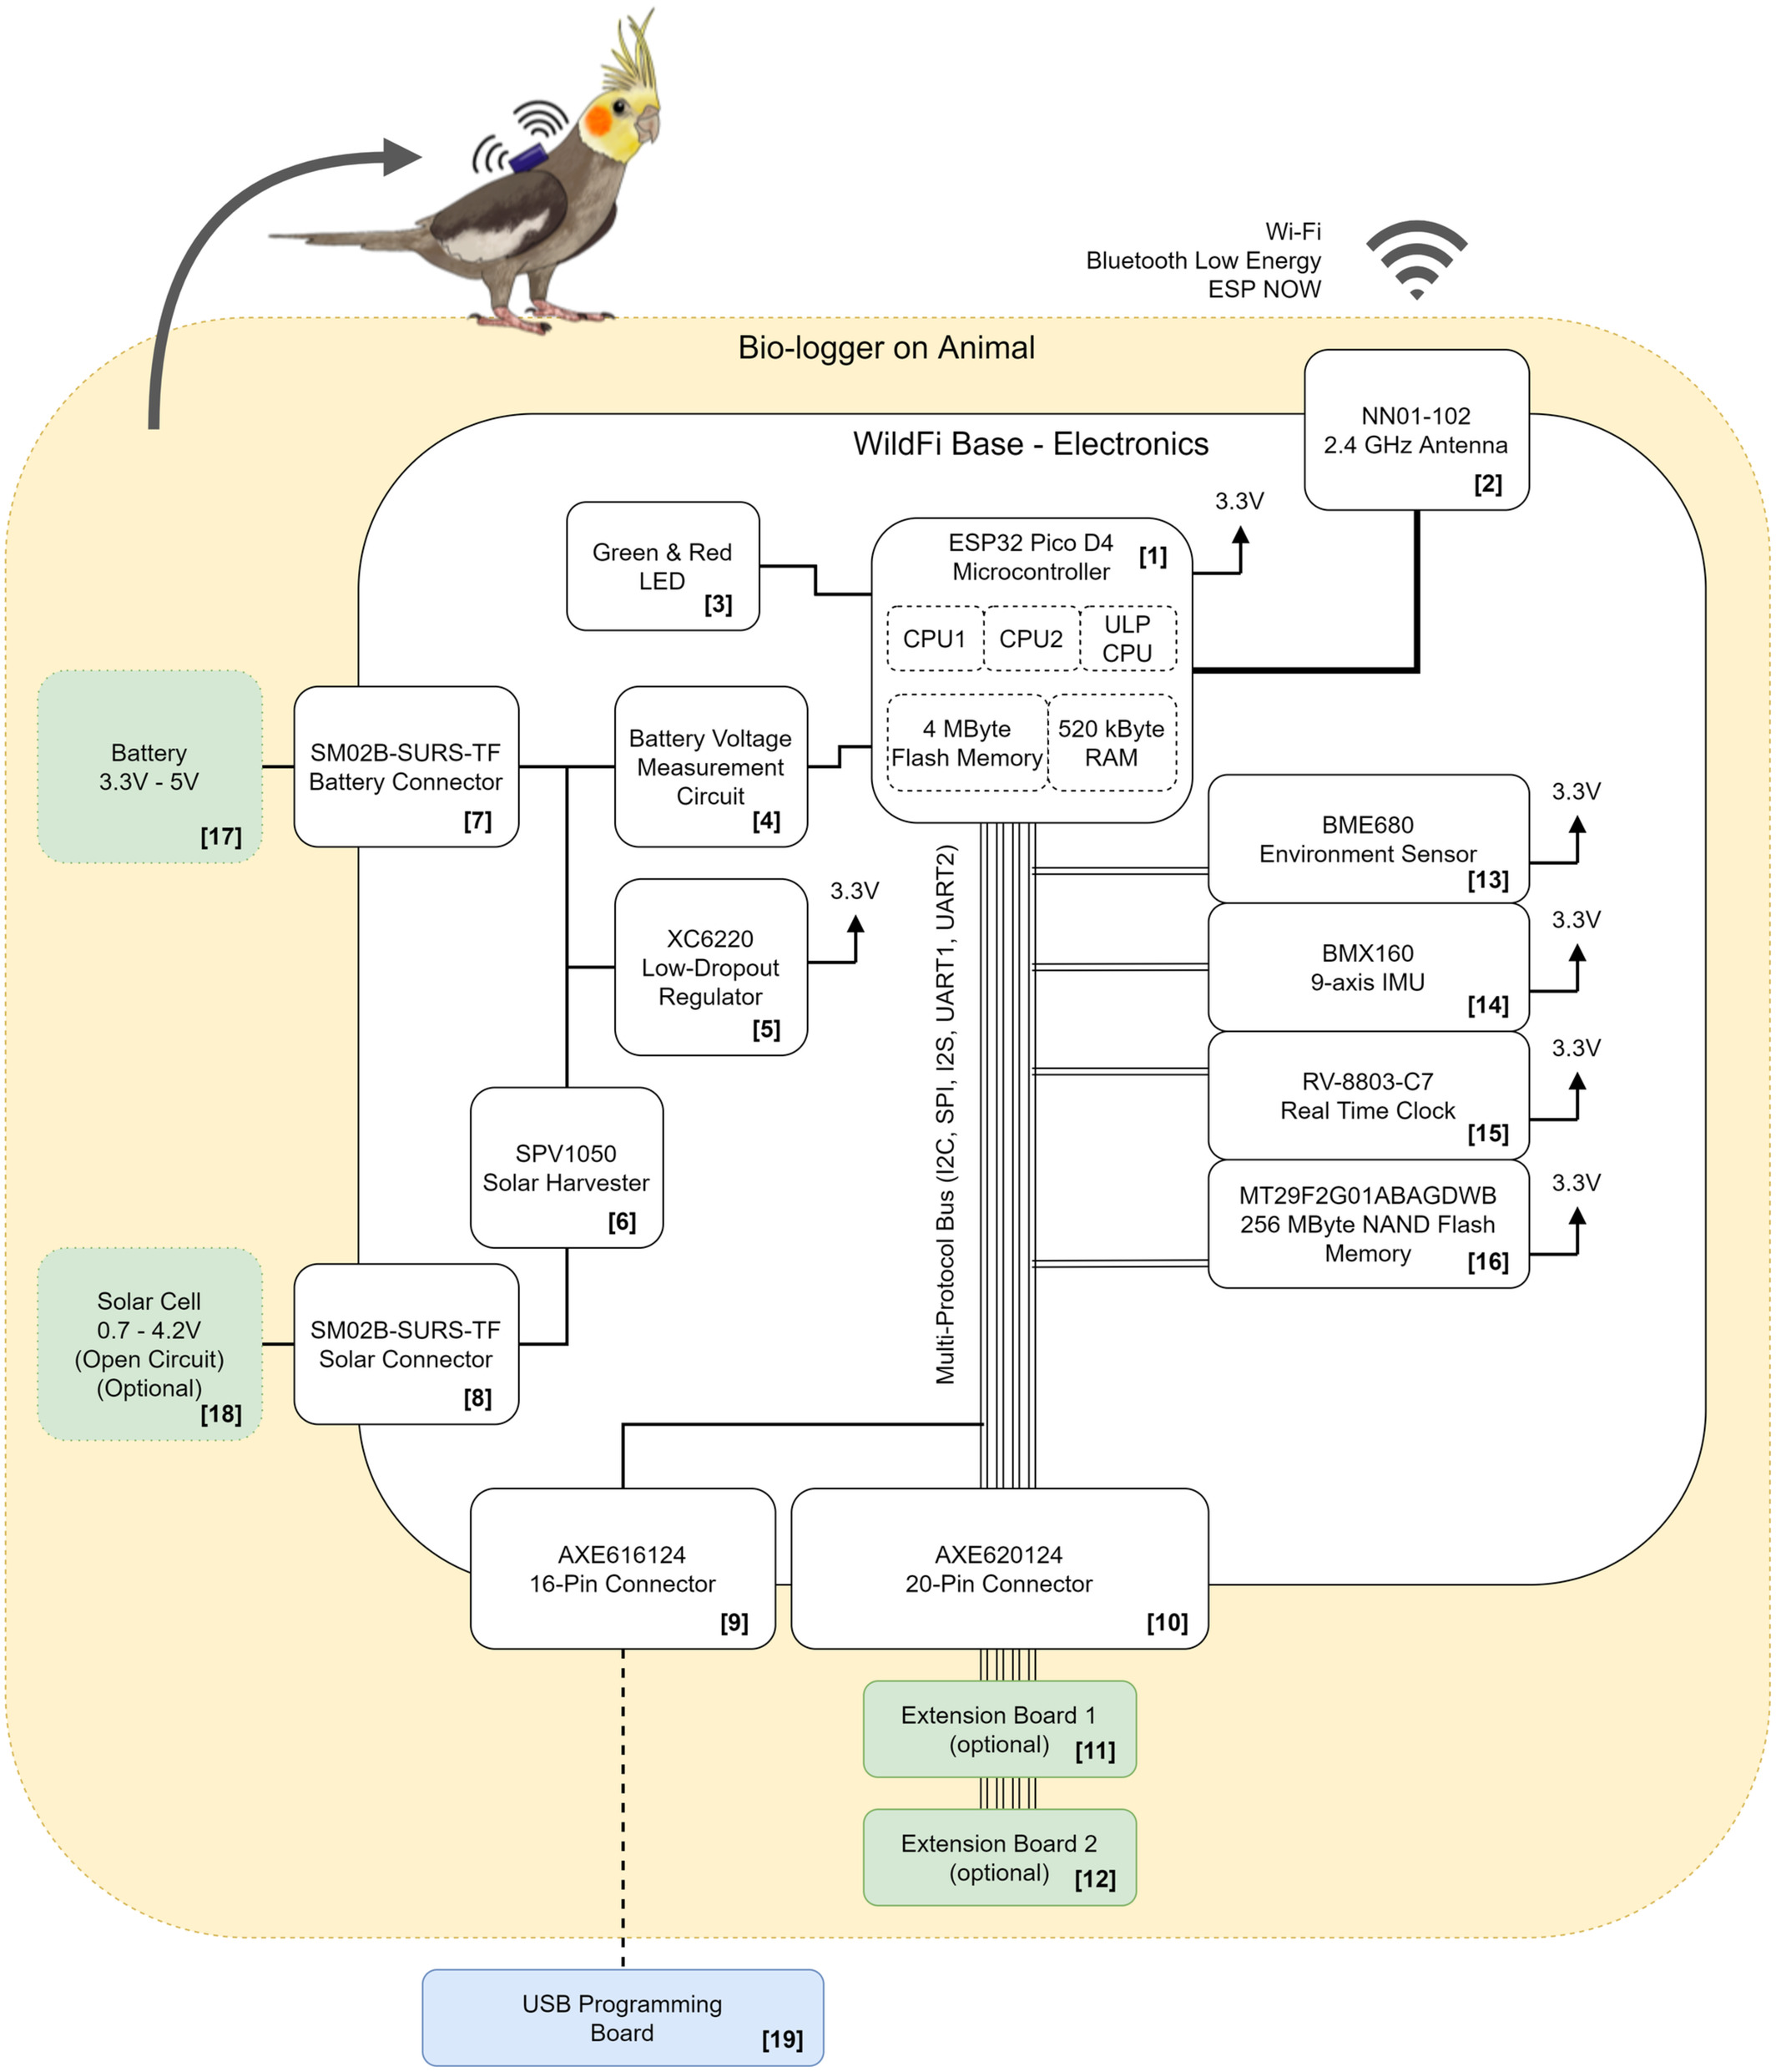
\includegraphics[width=.9\columnwidth]{images/wildfi_microcontroller.jpg}}
  \caption{SigFox network infrastructure\cite{wild2023internet}}
  \label{fig:WildFi_microcontroller}
\end{figure}
A power source is required for all of the components to work. Lithium polymer (LiPo) rechargeable batteries and 
dry batteries like AA/AAA/AAA can all be used to power the sensor devices. As long as a battery connector exists 
for the microcontroller of choice, anything can be used. Size and capacity are important factors to take into 
consideration when choosing a battery. A small battery format is likely to be preferred to reduce the effects the 
sensor devices may have on the animals function, but a sufficient capacity is also important in order to maintain 
operation for an extended period of time. A popular strategy used to address this problem is the use of solar 
energy harvesters to recharge the batteries; rechargeable batteries are a prerequisite for this setup. This allows 
for a smaller battery to be used while still maintaining an impressive battery life. How a solar harvester connects 
with a greater sensor system can be seen in figure ~\ref{fig:WildFi_microcontroller}, [18].
A biologging device is just a small computer without at least one sensor attached. There are many different types of 
sensors with different functions that can be attached to a microcontroller; so long as a given sensor has a way to be 
connected to a specific microcontroller, it can likely be used. The purpose of all of the various sensors is 
to collect data on the environment of the animal wearing the sensor device. This could mean locational data via GPS,   
temperature, air pressure and other meteorologic data via environment sensors and more. The number and types of sensors 
used in a sensor device will depend on what is of interest and there is a consideration of how many sensors can be 
implemented while maintaining a reasonable size. How sensors connect with a greater sensor device system can 
be seen in figure ~\ref{fig:WildFi_microcontroller}, [13, 14, 15].

\subsection{Gateway Devices}
\label{subsec:Gateway Devices}

The gateway devices of an IoT based biologging system falls within the networking layer of the IoT 
structure discussed in section ~\ref{subsec:What is the Internet of Things}. This means it is responsible 
for shuttling information to and from the perception and application layers. To complete this task, four main 
hardware components and requirements must be met: RF receiver/transmitter, data forwarding engine, power source, 
and connection to internet or greater local storage.
The RF (Radio Frequency) receiver/transmitter is a crucial component of the gateway device in a biologging system. 
It serves the purpose of communicating wirelessly with the sensor devices attached to the animals or objects being 
tracked. These RF modules receive data from the sensor devices and transmit commands or data to them as needed. 
These devices operate on specific frequencies that will depend on the network that is being used, the frequencies 
relevant to the biologging systems discussed in this paper can be found in sections ~\ref{subsec:Traditional Wifi 
(WLAN)} and ~\ref{subsec:Low Power Wide Area Networks (LPWAN)}.
The data forwarding engine within the gateway device manages the flow of data between the sensor devices and 
the external networks or storage systems. In some cases, the data forwarding engine may dump data into a local storage 
device or send it to the cloud via an internet connection. It processes incoming data from the RF receiver/transmitter, 
applies any necessary protocols or formatting, and forwards it to the appropriate destination. This component may include 
microcontrollers or specialized chips designed for efficient data handling and network communication.
A reliable power source is essential for the uninterrupted operation of the gateway device in a biologging system. 
Depending on the deployment scenario, power may be supplied through various means, including batteries, solar panels, 
or grid based power. The choice of power source depends on factors such as the duration of deployment, 
environmental conditions, resource availability, and power consumption of the gateway device. Efficient power management 
strategies are employed to maximize the device's uptime while minimizing energy consumption and the need for frequent 
maintenance. The designers of the WildFi tags utilized USB power banks and car batteries to power a gateway device for 
weeks\cite{wild2023internet}. 
The gateway device must have connectivity to either the internet or local storage to facilitate the transmission and 
storage of data collected from the sensor devices. In scenarios where real-time monitoring or remote access is required, 
an internet connection is necessary for transmitting data to cloud-based servers or remote databases. Alternatively, in 
environments with limited or intermittent internet access, the gateway device may store data locally on onboard storage 
devices such as flash memory or hard drives. This local storage option ensures data integrity and allows for later 
retrieval and analysis when connectivity is restored. For example, the ESP32 CAM development boards that the creators 
of the WildFi devices used as a foundation for a gateway device can store data locally on a SDHC memory card (up to 16GB) 
\cite{wild2023internet}.

\section{Networking}
\label{sec:Networking}

The networking of a IoT based biologging system is crucial in ensuring safe and
efficient data transmission. The networks used in a biologging system
are responsible for transmitting data from the perception layer to the application
layer, and are also responsible for ensuring that the data is transmitted
safely and securely. LPWAN and WLAN are two types of networks that are commonly used for 
biologging and each have their own advantages and disadvantages; the choice of which 
network to use is dependent on the specific use case. These networks must be able to transmit data over 
long distances, and they must be able to do so securely. The security 
of the data is especially important in a biologging system, as the data being 
transmitted is often sensitive and can be used to track the location of an animal, 
which in the hand of an illegal hunter, could be disastrous.

\subsection{Low Power Wide Area Networks (LPWANs)}
\label{subsec:Low Power Wide Area Networks (LPWANs)}

LPWAN provides a many benefits compared to WLAN, 
the primary benefits being that LPWANs are able to transmit data over much 
longer distances than WLANs with lower power consumption. This is especially beneficial 
in a biologging system, as the animals being tracked are often in vast, remote areas with battery powered sensor devices. 
LPWAN networks utilize sub 1GHz frequencies that require much less energy to transmit signals \cite{yousuf2018throughput}. LPWANs use 
unlicensed industrial, scientific and medical radio frequencies (ISM): these frequencies 
are set aside by governments across the globe for industrial, scientific and medical use. 
LPWANs utilize frequency modulation techniques in order to achieve ranges upwards of 40km and 
low power consumption. The SigFox proprietary network and LoRa standards based networks are 
two popular LPWANs that are explored further in subsections \ref{subsec:SigFox} and 
\ref{subsec:LoRa}.

\subsubsection{SigFox}
\label{subsec:SigFox}

The SigFox network is a proprietary LPWAN 
network that is used for IoT systems, and it can be used to cover an area as 
big as Belgium ($30,600 km^2$) with only seven base stations \cite{wild2023multi}. 
The node device in a SigFox network is able to transmit 6 messages per hour, 
each having a maximum size of 12 bytes. While 12 bytes may seem limiting, it is 
sufficient for transmitting the GPS coordinates of an animal, as well as other 
sensor data such as temperature\cite{wild2023multi}. The SigFox company also offers 
the Atlas technology which uses the signal strength and location of the receiving 
base station to calculate an approximate location of the node device, which frees up 
the node device from having to explicitly send GPS data, allowing for other sensor data 
to be sent instead\cite{wild2023multi}. 
\begin{figure}[htbp]
  \centering
  \fbox{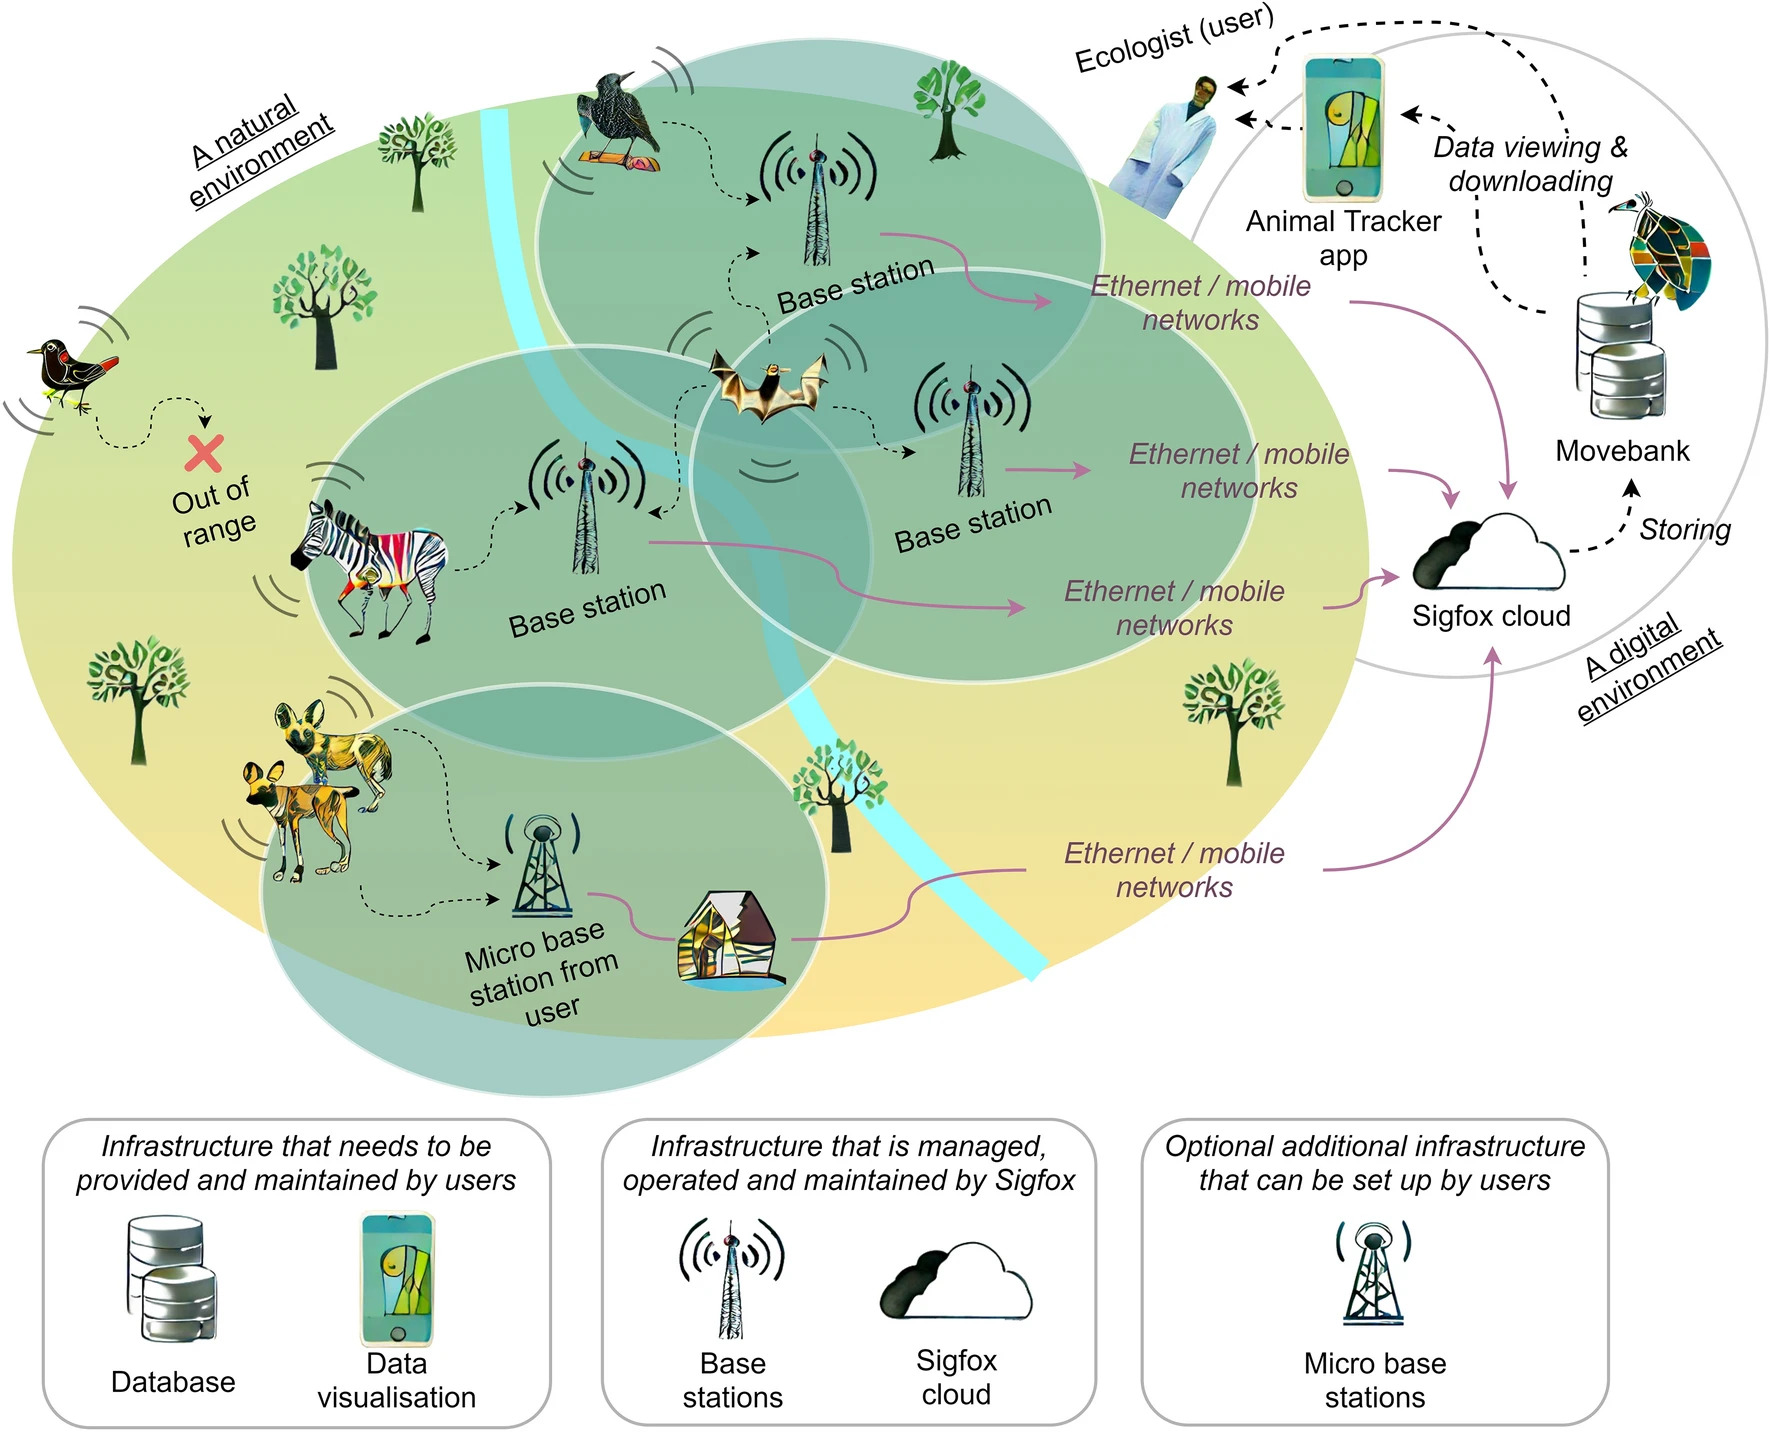
\includegraphics[width=.9\columnwidth]{images/SigfoxNetworkMap.jpg}}
  \caption{SigFox network infrastructure\cite{wild2023multi}}
  \label{fig:SigFox_infrastructure}
\end{figure}
SigFox uses frequency hopping modulation which transmits data three 
times at different frequency channels at different times, which ensures a message is received 
and robustness to interferences \cite{LavricSigfoxCommunication}. Using the specifications of SigFox's 
network, a sensor device is able to send 140 packets per day with power consumption  
between 19 and 49 mA, two AAA batteries are able to power a node up to 6.5 years
\cite{LavricSigfoxCommunication}. Because SigFox is a proprietary network, end users 
do not maintain the base stations or connection to the SigFox cloud: they only need to 
design their devices within the SigFox specifications and connect them to the SigFox network. 
An overview of the SigFox infrastructure and how it can be applied to biologging 
is shown in Figure ~\ref{fig:SigFox_infrastructure}.

\subsubsection{LoRa}
\label{subsec:LoRa}

LoRa is a standards based LPWAN; this means that sensor and gateway devices can be self developed and deployed 
as long as the LoRa alliance standards are followed \cite{LoRa_Alliance®_2023}; There are also public LoRa networks 
available for use in the case where a user just wants to design the sensor device.
The LoRa standards utilize CHIRP (Compressed High Intensity Radar Pulse) spread 
spectrum transmission modulation. CHIRP is different from the frequency hopping technique that the SigFox 
network uses. Instead of transmitting at a constant frequency and then hopping to a different frequency, 
CHIRP modulates by increasing or decreasing it's frequency over time, this can be done both linearly or not \cite{ghoslya2017lora}. The 
spreading factor determines how quickly this modulation takes place; LoRa uses spreading 
factors SF7 to SF12, the larger the spreading factor, the slower the modulation.
How these spreading factors compare to each other is shown in Figure ~\ref{fig:Chirp}. 
The main tradeoffs between spreading factors is the range and data rate of the network, as the 
spreading factor increases, the range of the network increases, but the data rate decreases \cite{erturk2019survey}.
\begin{figure}[htbp]
  \centering
  \fbox{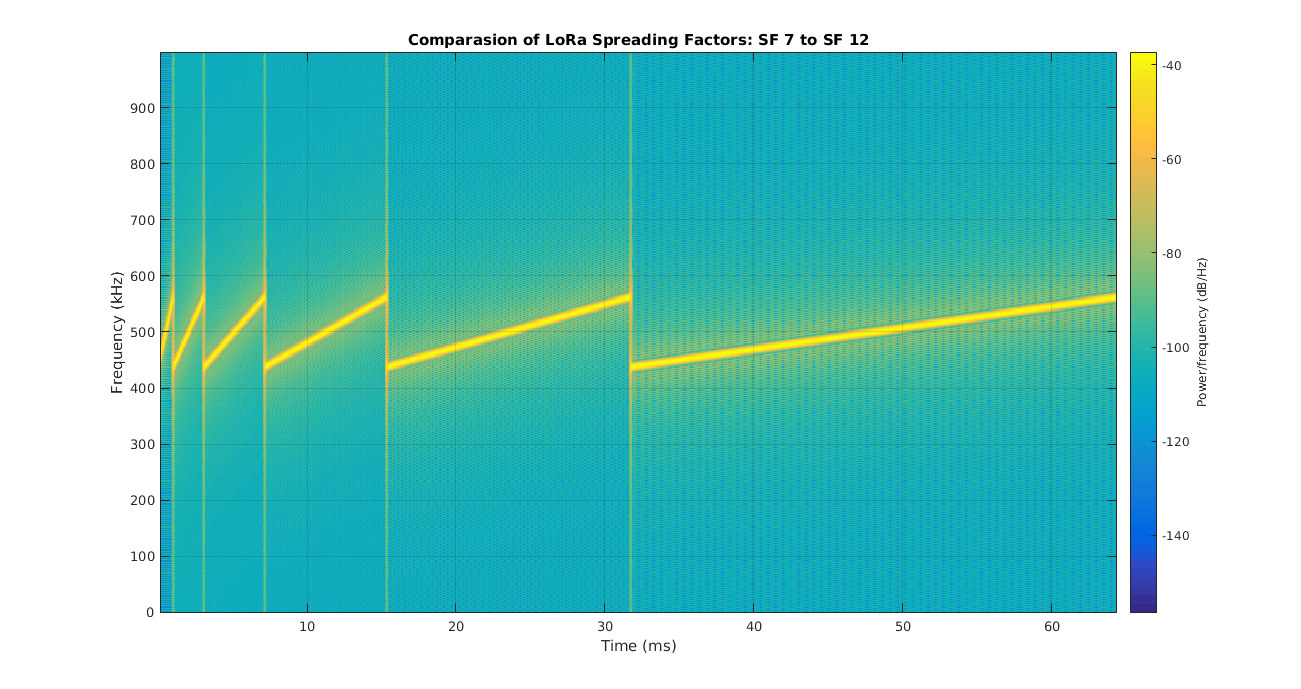
\includegraphics[width=.9\columnwidth]{images/Chirp.png}}
  \caption{Chirp Spread Spectrum Spreading factors\cite{ghoslya2017lora}}
  \label{fig:Chirp}
\end{figure}
The spreading factor then becomes a critical factor in the design of a LoRa network, as 
the spreading factor is directly related to the range and data rate of the network, so it should 
be chosen wisely to fit the needs of the specific use case. Because the frequency is constantly 
increasing or decreasing, chirp is able to tolerate interference better than that of the frequency hopping 
technique that the SigFox network uses.

\subsection{Wireless Local Area Networks (WLAN)}
\label{subsec:Wireless Local Area Networks (WLAN)}

A WLAN is another method that is used by some ecologists to 
implement biologging systems. There are some useful benefits to using a WLAN over an LPWAN; The biggest of which is data 
transfer rate. However, because WLAN uses 2.4/5/6GHz frequencies, the range is much more limited 
than that of a LPWAN network, and the power consumption is higher. The WildFi biologging system designed by 
Timm Wild and his colleagues is just one example of a device that uses traditional 
WLAN to collect data from a biologging device. Wild is also a leading member of the 
team that studied the use of the SigFox network for a IoT based biologging system, and 
claimed that the data transmission capacity was one of the reasons that they chose to 
investigate the use of a WLAN for biologging \cite{wild2023internet}. 
The WildFi tags and others like it, connect and communicate by using a traditional wireless 
routers, smartphone hotspots or homemade gateway devices, which provides a versatile way for tags to offload collected data; 
these capabilities can be seen in Figure ~\ref{fig:wild-fi_IoT_diagram}.
\begin{figure}[htbp]
  \centering
  \fbox{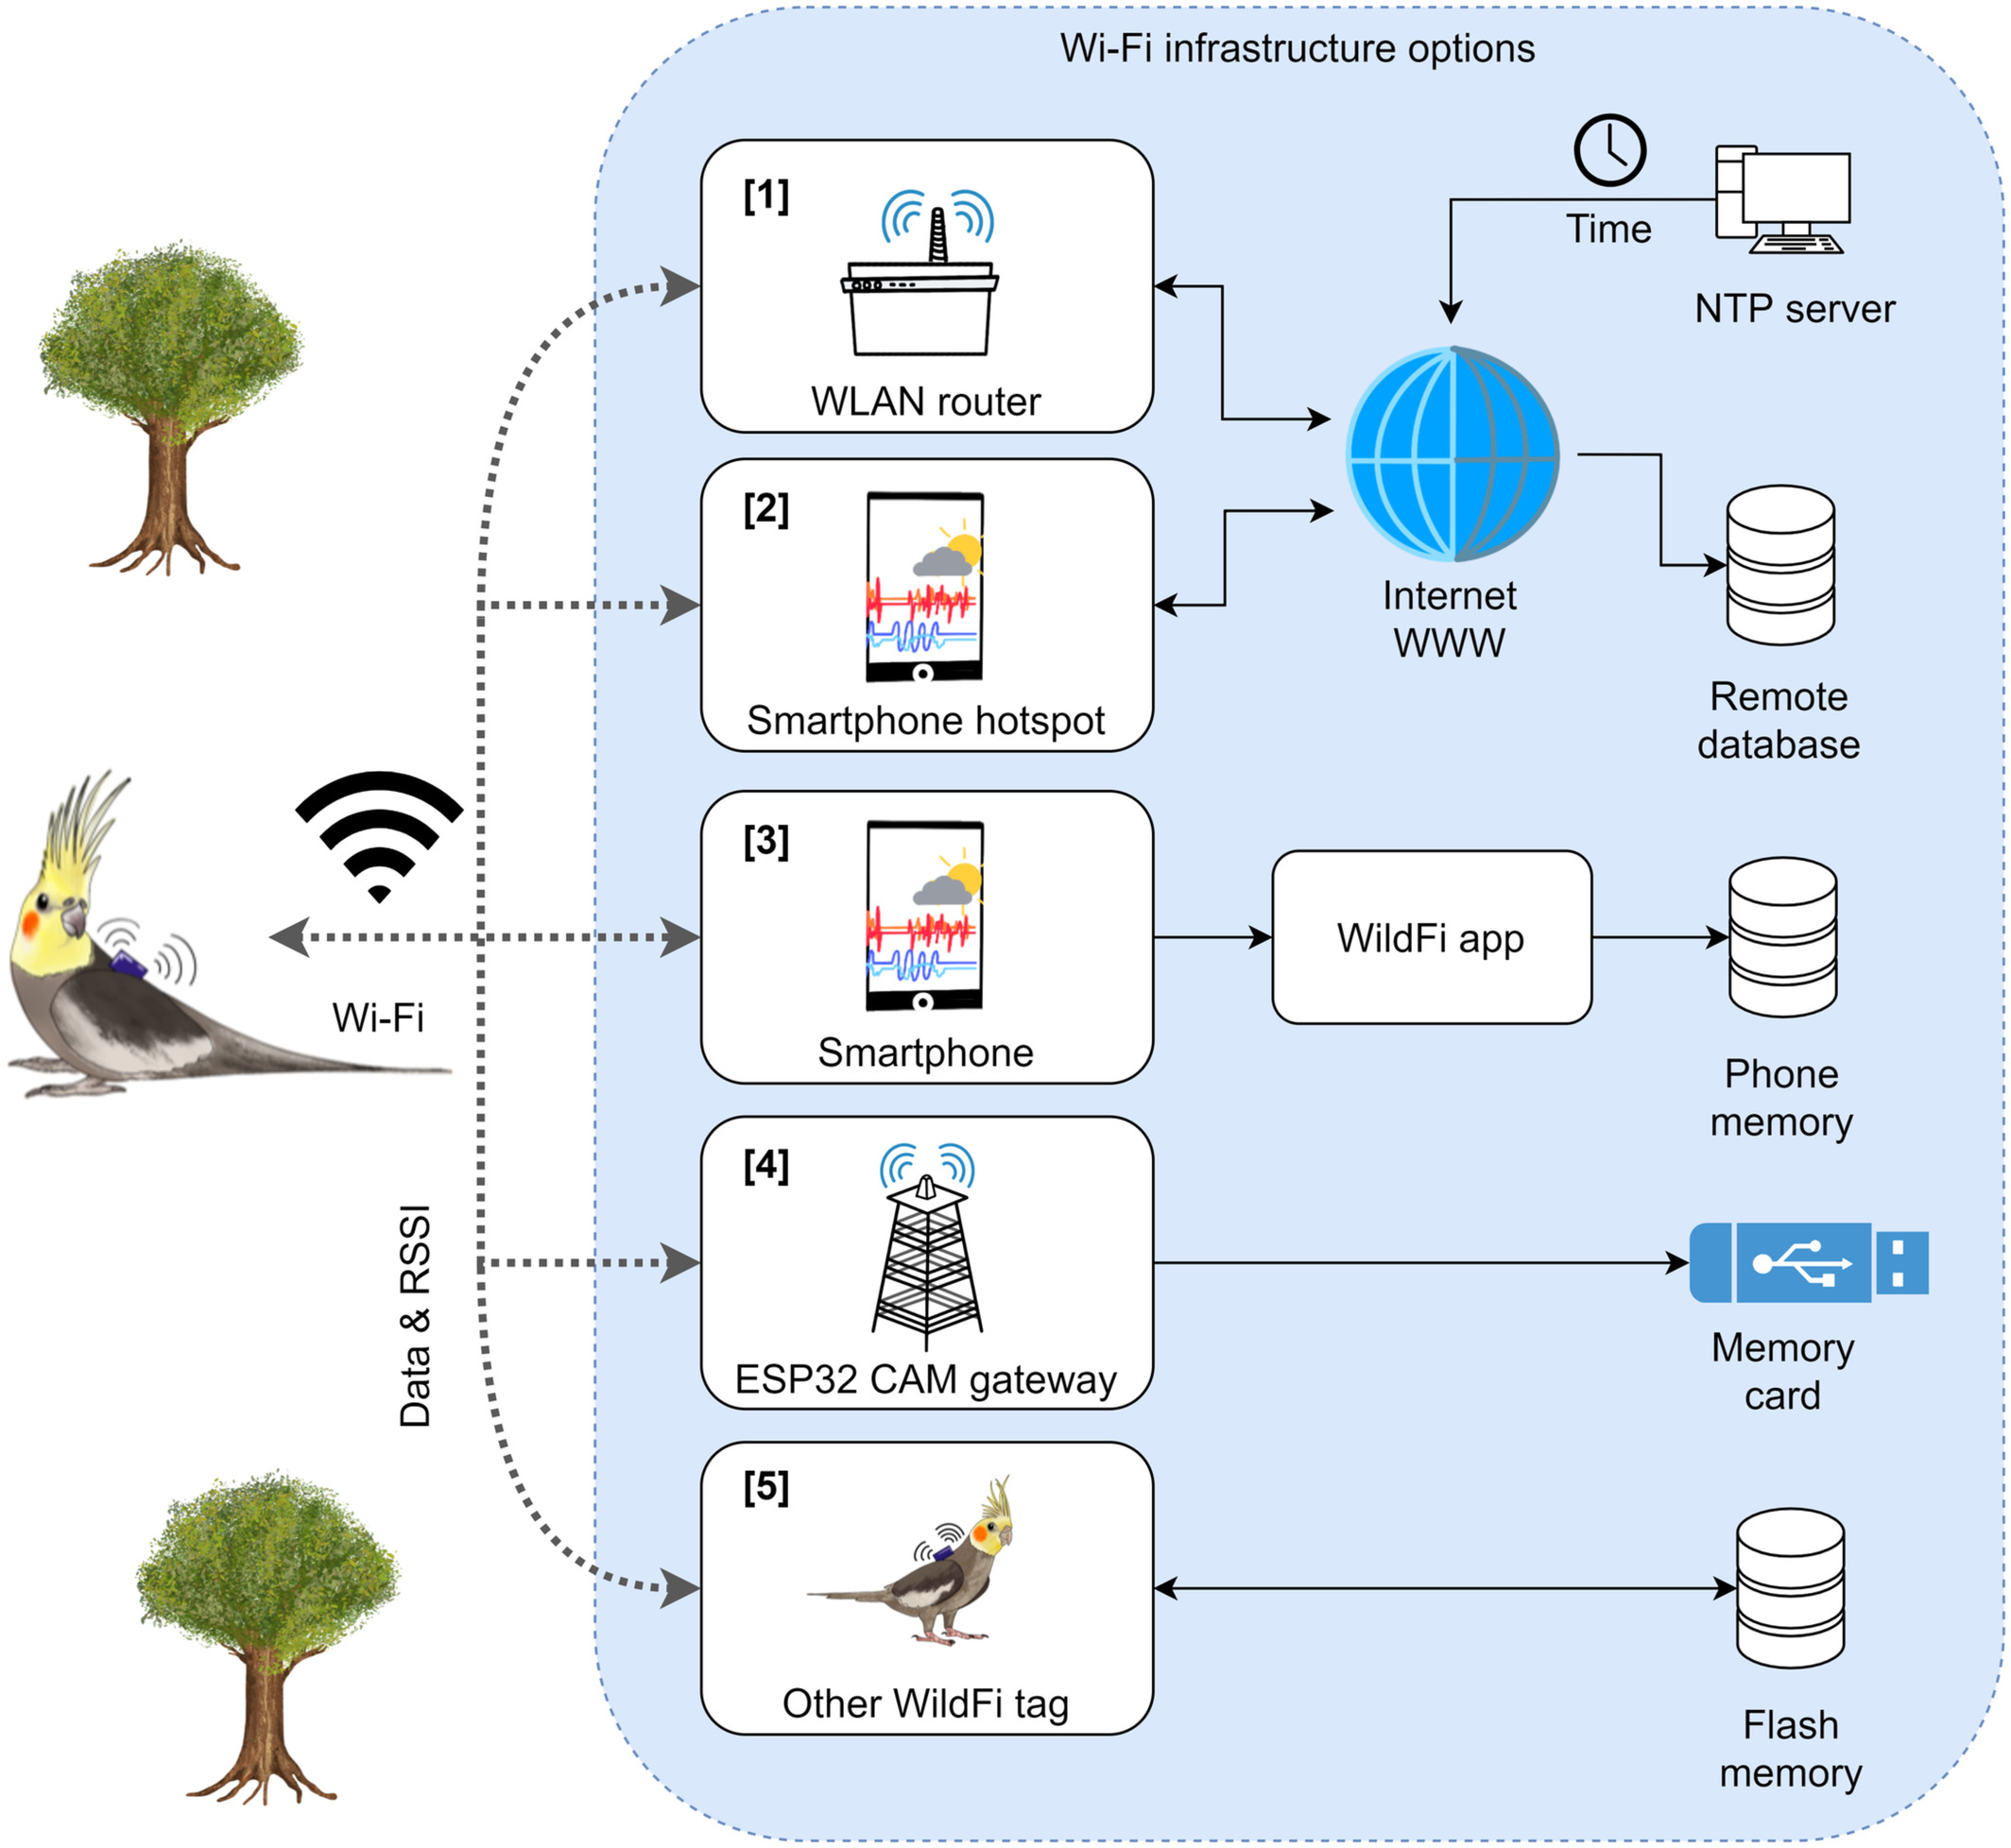
\includegraphics[width=.8\columnwidth]{images/WildFi_IoT.jpg}}
  \caption{Wild-fi IoT infrastructure overview \cite{wild2023internet}}
  \label{fig:wild-fi_IoT_diagram}
\end{figure}
WLAN biologging have higher power consumption than a LPWAN based system, however the energy cost per byte 
transmitted is lower than a LPWAN based device, and Wild et. al claim that using a logging device that has a 
70mAh battery and a small solar panel, data can be transmitted 24 hours a day for an entire lifetime of an animal \cite{wild2023internet}.

\subsection{Security}
\label{subsec:Security}

The security of these networks is a critical factor in the design of a biologging system, as 
the data being transmitted is often sensitive and can be used to track the location of an animal, 
which in the hand of an illegal hunter, could be disastrous. While much of the security of the 
data is in the design of the physical device and it's software, the networks being used also need to 
be secure and safe. The security of the physical device is important in the event that a sensor 
device is lost or stolen; typically, this is done by having per device keys to ensure that if a 
device is compromised, it won't hurt any other devices on the network.

\subsubsection{SigFox and LoRa Security}
\label{subsec:SigFox and LoRa Security}

Both the SigFox and LoRa network ensure safe data transmission by using AES (Advanced Encryption Standard) 
128 for end-to-end encryption. With this encryption method, a 128 bit key is used to encrypt the data from 
sensor device and a key is shared with the application server so that it can decrypt the data \cite{AES128IoT}. 
This ensures that the data is encrypted at the source, encrypted in transit, and decrypted at the destination. 
This is important for the security of the data, as it prevents the data 
from being readable by anyone who has access to the data. There are many benefits to using AES 128 for end-to-end encryption, including 
it's proven track record for being secure and efficient. Compared to other encryption methods, AES 128 
has a small encryption key which makes it less computationally intensive; This leads into another reason why 
it was chosen for use in these two LPWAN networks. Due to it being computationally efficient, it is 
a great choice for a system designed around being low power. For a deeper dive into AES 128 encryption and 
how it is used in LPWAN networks refer to Kun-Lin Tsai's article on the matter \cite{AES128IoT}.

\subsubsection{WLAN Security}
\label{subsec:WLAN Security}

The security mechanisms of a IoT based biologging device that uses a traditional Wifi network can vary 
depending on the developer of each device and their own preference on how to safely transmit data to the gateway 
device. In the case of the WildFi devices discussed in section ~\ref{subsec:Wireless Local Area Networks (WLAN)}, data 
transmissions are encrypted with WPA2 and HTTPS \cite{wild2023internet}. These two methods allow for ease of 
use for the developer because they are widely supported by most WLAN devices that would be used as gateway 
devices. WPA2 and HTTPS, similar to the LPWAN networks, uses AES 128 encryption to some extent, this provides the same 
benefits as previously discussed \cite{WPA2Moissinac}. 

\subsection{Comparison and Selection Criteria}
\label{subsec:Protocol Comparison and Selection Criteria}

Examining the benefits and pitfalls of each IoT network in relation to what is important in a biologging 
system is important to understand what network to choose for a given application. While many factors are 
important when accessing these networks for capabilities as IoT network solutions, range, data rate, battery 
life and security will be the focus of this comparison because they are the most critical for a biologging 
system. Each network discussed in section ~\ref{sec:Networking} offers different levels of ability in each 
of these categories: I rank their abilities in figure ~\ref{fig:network_barplot}. This figure gives a good 
idea of how the three networks compare to each other in the five critical categories. Table ~\ref{table:Network_Comparison_Table} 
lays out how the three networks compare numerically: important rows in this table are the data rate and range rows.
Ultimately, the best network will depend on availability of public networks and the technical knowhow and ability of the user. 
If the user is not capable of creating their own network and devices, then a solution like SigFox or LoRa 
may be a better choice. On the other hand, if a user can develop their own system, there are some serious 
benefits to using LoRa or WLAN, mainly data rate and cost. Each use case for a biologging system is 
unique and the network of choice will mostly depend on what is needed to meet the demands of the specific 
use case.
\definecolor{MineShaft}{rgb}{0.2,0.2,0.2}
\definecolor{Silver}{rgb}{0.752,0.752,0.752}
\begin{table}
\centering
\begin{tblr}{
  width = \linewidth,
  colspec = {Q[177]Q[285]Q[285]Q[185]},
  row{3} = {fg=MineShaft},
  row{4} = {fg=MineShaft},
  row{5} = {fg=MineShaft},
  row{6} = {fg=MineShaft},
  cell{2}{2} = {fg=MineShaft},
  cell{2}{3} = {fg=MineShaft},
  cell{2}{4} = {fg=MineShaft},
  hlines = {Silver},
  vlines,
  hline{1-2,7} = {-}{black},
}
                     & SigFox                             & LoRa                               & WLAN                  \\
Frequency            & 868MHz(EU) / 915MHz(NA) / 433MHz(AS) & 868MHz(EU) / 915MHz(NA) / 433MHz(AS) & 2.4GHz/ 5GHz/ 6GHz      \\
Data Rate            & 100bps                             & 50kbps                             & 1840kbps              \\
Maximum messages/day & 140                                & Unlimited                          & Unlimited             \\
Range                & 10 km (urban), 40 km (rural)       & 5 km (urban), 20 km (rural)        & 200m                  \\
Security             & AES-128                            & AES-128                            & WPA2/ HTTPS (AES128) 
\end{tblr}
\caption{Characteristics of explored networks, data from \cite{mekki2019comparative} and \cite{wild2023internet}}
\label{table:Network_Comparison_Table}
\end{table}

\begin{figure}[htbp]
  \centering
  \fbox{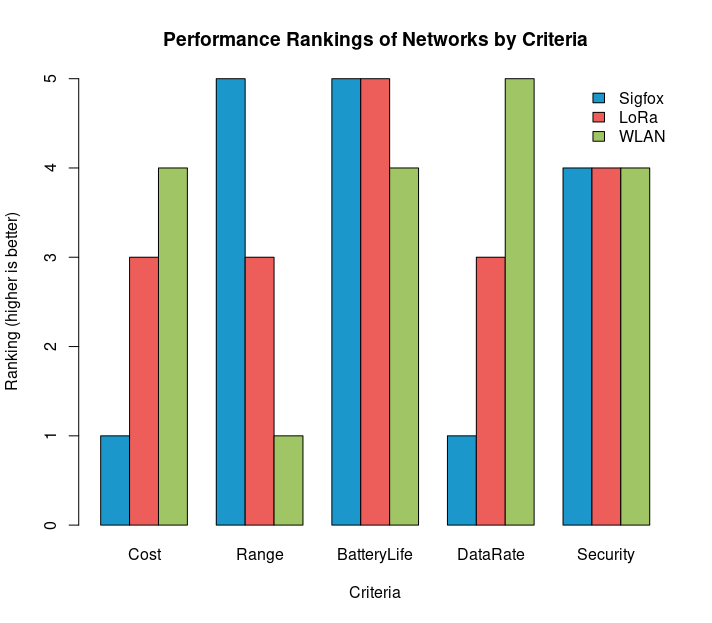
\includegraphics[width=.9\columnwidth]{images/Network_Comparison_barplot.png}}
  \caption{Rankings of discussed networks under 5 critical criteria (5=better, 1=worse)}
  \label{fig:network_barplot}
\end{figure}

\section{Closing Statements}
\label{sec:Closing Statements}

\subsection{Ethical Considerations}
\label{sec:Ethical Considerations}

Biologging raises some ethical concerns for a few reasons. First, animals must first be captured so that a sensor device can be 
attached. In any case this will increase the stress on the animal, and it can be argued that this is necessary for ecologists to understand the animal. 
Fortunately, the use of IoT based biologging means that this only has to happen once, and the data is automatically retrieved rather than manually 
collected. Another concern is that with increased popularity and decreased cost, that too many animals will have electronic tags on them. This is a 
real concern, however this is something that can be prevented by requiring permits or licenses to tag animals.

\subsection{Conclusion}
\label{sec:Conclusion}

In conclusion, the integration of IoT technologies with biologging systems presents unprecedented opportunities for 
advancing wildlife tracking and ecological research. The exploration of Low Power Wide Area Networks (LPWAN) such 
as SigFox and LoRa, alongside traditional WiFi networks, underscores the importance of selecting the most suitable 
networking protocol based on the specific requirements of the application. Moreover, robust security measures, coupled 
with advancements in sensor technology and data transmission, offer promising avenues for enhancing the efficiency 
and reliability of biologging systems. As we continue to innovate and refine these technologies, the future of 
wildlife monitoring holds immense potential for gaining deeper insights into animal behavior, and contributing to 
conservation initiatives.

%%
%% The acknowledgments section is defined using the "acks" environment
%% (and NOT an unnumbered section). This ensures the proper
%% identification of the section in the article metadata, and the
%% consistent spelling of the heading.
\begin{acks}
  TODO
\end{acks}

%%
%% The next two lines define the bibliography style to be used, and
%% the bibliography file.
\bibliographystyle{ACM-Reference-Format}
\bibliography{CBeaneSeniorSem}


\end{document}
\endinput
%%
%% End of file `sample-sigplan.tex'.
